\setchapterpreamble[u]{\margintoc} 
\chapter{Corriger un SLCI} 
\section{Analyser un choix de correcteur (compensation de pôles, nombre d'intégrations)} 
\section{Régler un correcteur P graphiquement ou analytiquement} 
\graphicspath{{\repStyle/png/}{../COR/COR-02-P/65_Eclipse/images/}} 
\normaltrue \difficilefalse \tdifficilefalse
\correctionfalse
%\UPSTIidClasse{11} % 11 sup, 12 spé
%\newcommand{\UPSTIidClasse}{11}

\exer{Système éclipse $\star$ \label{C2:04:65}}
% Banque PT SI A 2009
\setcounter{question}{0}
\marginnote{\xpComp{COR}{02}}%\UPSTIcompetence[2]{C2-04}
\index{Compétence C2-04}
\index{Compétence C2OR-02}
\index{Correcteur}
\index{Correcteur proportionnel}
\index{Système éclipse}


\ifcorrection
\else
\marginnote{\textbf{Pas de corrigé pour cet exercice.}}
\fi

\ifprof
\else 

Le schéma-blocs sous la forme suivante avec un gain unitaire pour le capteur
de vitesse.

\begin{center}
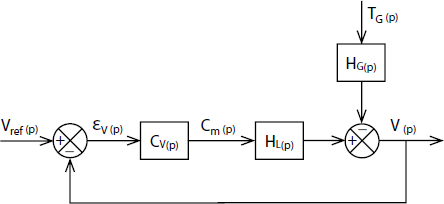
\includegraphics[width=\linewidth]{65_01}
\end{center}

$H_L(p)=\dfrac{K_L}{1+\tau_L p}$ et $H_G(p)=\dfrac{K_G}{1+\tau_G p}$  avec $\tau_G=\tau_L = \SI{20}{ms}$, $K_L = \SI{1e-3}{N^{-1}s^{-1}}$ et $K_G = \SI{2e-5}{mN^{-1}s^{-1}}$.


Le cahier des charges donne les valeurs des critères d'appréciation adoptés :
\begin{itemize}
\item la précision : en régime permanent à vitesse constante, soit $\varepsilon_S=0$ et à accélération constante, soit $\varepsilon_T=0$; $\varepsilon_S$ désigne l'erreur statique de position et $\varepsilon_T$ l'erreur statique de vitesse ou erreur de traînage;
\item la rapidité : le temps de réponse à \SI{5}{\%} tel que : $t_{\text{R}\SI{5}{\%}}\leq \SI{1}{s}$;
\item la stabilité : marge de phase $\geq \SI{45}{\degres}$ et marge de gain $\geq \SI{10}{dB}$.
\end{itemize}

On choisit tout d'abord une correction proportionnelle telle que $C_V(p)=K_P$.
\fi

\question{Le cahier des charges est-il respecté en termes de précision, rapidité et stabilité ?}
\ifprof
\else 
\fi

\question{Peut-on choisir une valeur de $K_P$ qui puisse assurer le respect complet du cahier des charges ?}
\ifprof
\else 
\fi

\question{Le système est-il robuste à une perturbation en échelon ?}
\ifprof
\else 
\fi

\ifprof
\else

\noindent\footnotesize
% \fbox{\parbox{.9\linewidth}{
% Éléments de corrigé : 
% \begin{enumerate}
  % \item $\varepsilon_{\text{con \%}} = \dfrac{1}{1+K_PK_m K_{\text{pom}} K_{\text{cap}} }$;
  % \item $K_P > 19$;
  % \item $\varepsilon_{\text{pert}} = \Delta Q_e \dfrac{K_f}{1+K_{\text{cap}}K_PK_mK_{\text{pom}}}$;
  % \item $K_P > 2,19$.
  % \item $K_P < 0,125$. Il est impossible de vérifier les trois conditions avec un correcteur proportionnel.
% \end{enumerate}}}
\normalsize
\marginnote{Corrigé voir \ref{C2:04:65}.}
\fi 
 
\section{Régler un correcteur PI graphiquement ou analytiquement} 
\graphicspath{{\repStyle/png/}{../COR/COR-03-PI/65_Eclipse_02/images/}} 
\normaltrue \difficilefalse \tdifficilefalse
\correctionfalse
%\UPSTIidClasse{11} % 11 sup, 12 spé
%\newcommand{\UPSTIidClasse}{11}

\exer{Système éclipse $\star$ \label{COR:03::65:02}}
% Banque PT SI A 2009
\setcounter{question}{0}\marginnote{\xpComp{COR}{03}}%\UPSTIcompetence[2]{C2-04}
\index{Compétence C2-04}\index{Compétence COR-03}
\index{Correcteur}
\index{Correcteur intégral}
\index{Système éclipse}


\ifcorrection
\else
\marginnote{\textbf{Pas de corrigé pour cet exercice.}}
\fi

\ifprof
\else
Le schéma-blocs sous la forme suivante avec un gain unitaire pour le capteur
de vitesse.

\begin{marginfigure}
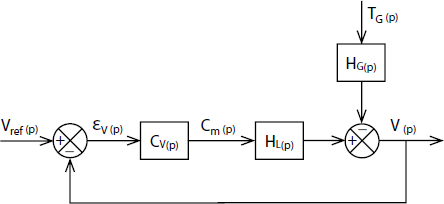
\includegraphics[width=\linewidth]{65_01}
\end{marginfigure}

$H_L(p)=\dfrac{K_L}{1+\tau_L p}$ et $H_G(p)=\dfrac{K_G}{1+\tau_G p}$  avec $\tau_G=\tau_L = \SI{20}{ms}$, $K_L = \SI{1e-3}{N^{-1}s^{-1}}$ et $K_G = \SI{2e-5}{mN^{-1}s^{-1}}$.


Le cahier des charges donne les valeurs des critères d'appréciation adoptés :
\begin{itemize}
\item la précision : en régime permanent à vitesse constante, soit $\varepsilon_S=0$ et à accélération constante, soit $\varepsilon_T=0$; $\varepsilon_S$ désigne l'erreur statique de position et $\varepsilon_T$ l'erreur statique de vitesse ou erreur de traînage;
\item la rapidité : le temps de réponse à \SI{5}{\%} tel que : $t_{\text{R}\SI{5}{\%}}\leq \SI{1}{s}$;
\item la stabilité : marge de phase $\geq \SI{45}{\degres}$ et marge de gain $\geq \SI{10}{dB}$.
\end{itemize}

On considère que le système n'est pas perturbé et que $T_G(p)=0$.
On choisit tout d'abord une correction intégrale telle que $C_V(p)=\dfrac{K_i}{p}$.
\fi

\question{Le cahier des charges est-il respecté en terme de précision ?}
\ifprof
\else 
\fi

\question{Calculer numériquement le temps de
réponse à \SI{5}{\%} optimal obtenu avec cette correction. Préciser la valeur de $K_i$ permettant d'obtenir ce temps de
réponse}
\ifprof
\else 
\fi

%\question{A-t-on augmenté ou diminué la rapidité du système par rapport à la correction proportionnelle ?}
%\ifprof
%\else 
%\fi

\question{Tracer l'allure du diagramme de Bode de la FTBO corrigée avec ce correcteur.}
\ifprof
\else 
\fi

\question{Indiquer la marge de phase.}
\ifprof
\else 
\fi

\question{Calculer la valeur de $K_i$ limite assurant le cahier des charges en terme de marge de phase.}
\ifprof
\else 
\fi

\question{Vérifier cette valeur en vous aidant du diagramme de Bode partiel de la fonction $C_V(p).H_L(p)$, donné  ci-dessous pour la valeur particulière : $K_i=7000$.}
\ifprof
\else 
\fi


\ifprof
\else
\begin{marginfigure}
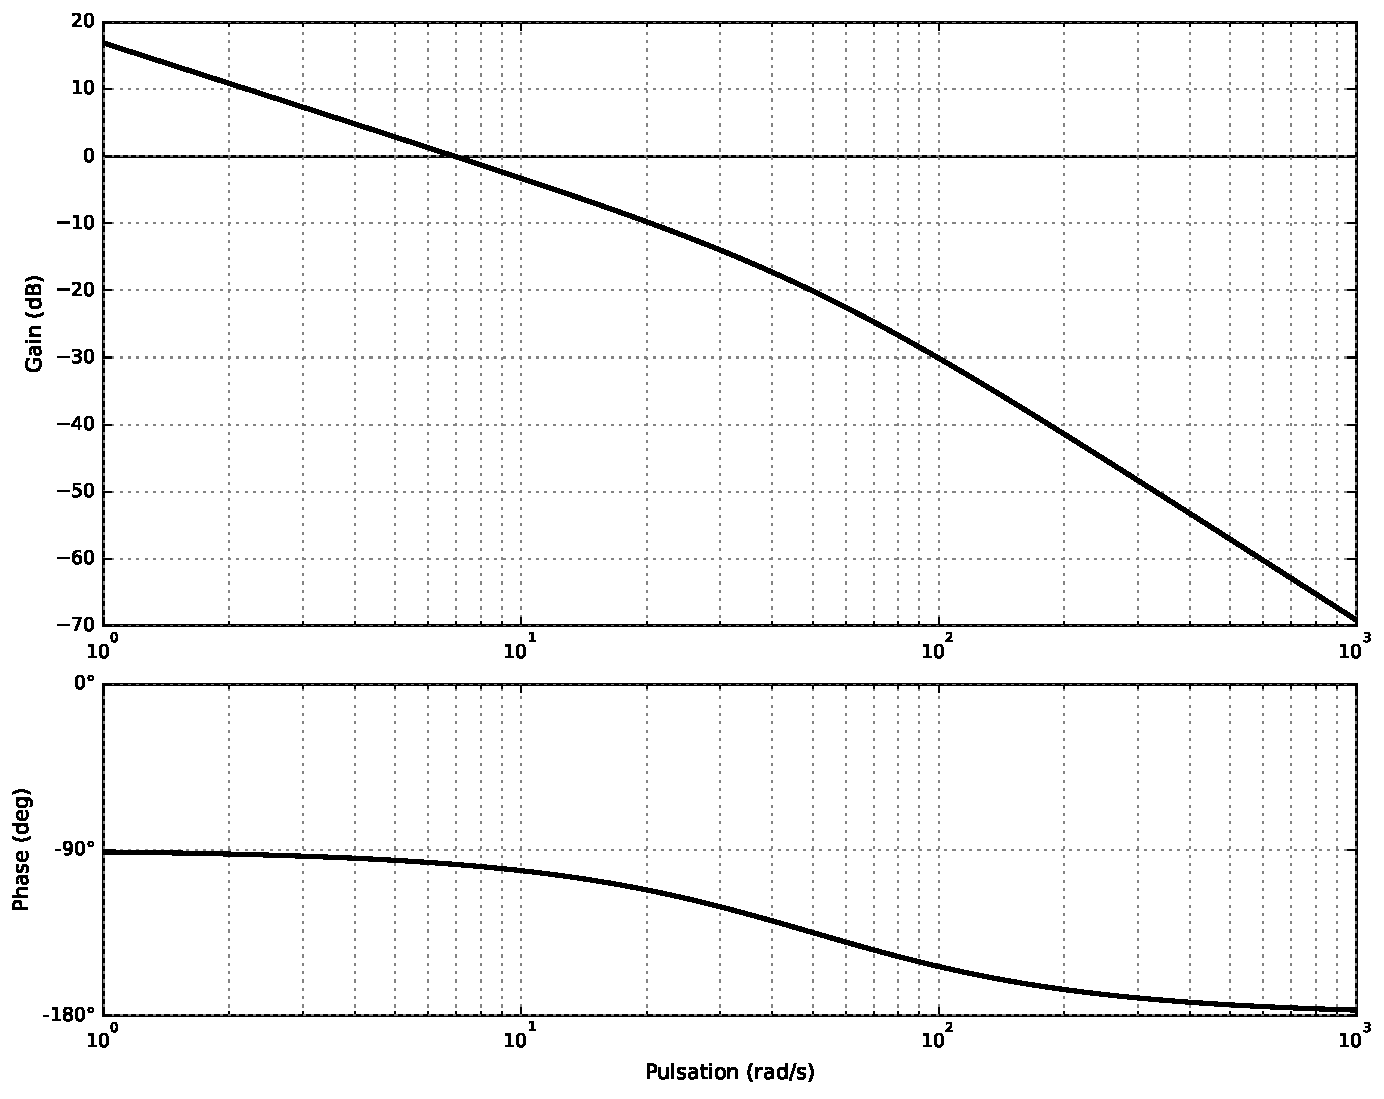
\includegraphics[width=\linewidth]{65_02}
\end{marginfigure}
\fi

\question{Que pensez vous de cette valeur, vis-à-vis du comportement du système, comparée à celle trouvée précédemment.}
\ifprof
\else 
\fi

\question{Un correcteur de type $C_V(p)=\dfrac{K_i}{p^2}$, permettrait-il d'obtenir les performances attendues en terme de précision et pourquoi ? }
\ifprof
\else 
\fi

\question{Permet-il d'assurer la stabilité du système et pourquoi ?}
\ifprof
\else 
\fi


\ifprof
\else

\noindent\footnotesize
% \fbox{\parbox{.9\linewidth}{
% Éléments de corrigé : 
% \begin{enumerate}
  % \item $\varepsilon_{\text{con \%}} = \dfrac{1}{1+K_PK_m K_{\text{pom}} K_{\text{cap}} }$;
  % \item $K_P > 19$;
  % \item $\varepsilon_{\text{pert}} = \Delta Q_e \dfrac{K_f}{1+K_{\text{cap}}K_PK_mK_{\text{pom}}}$;
  % \item $K_P > 2,19$.
  % \item $K_P < 0,125$. Il est impossible de vérifier les trois conditions avec un correcteur proportionnel.
% \end{enumerate}}}
\normalsize


\marginnote{Corrigé voir \ref{COR:03::65:02}.}

\fi 
 
\graphicspath{{\repStyle/png/}{../COR/COR-03-PI/66_Micromanipulateur/images/}} 
\normaltrue \difficilefalse \tdifficilefalse
\correctionfalse
%\UPSTIidClasse{11} % 11 sup, 12 spé
%\newcommand{\UPSTIidClasse}{11}

\exer{Micromanipulateur $\star$ \label{COR:03::66}}
% CCP PSI 2009
\setcounter{question}{0}\marginnote{\xpComp{COR}{03}}%\UPSTIcompetence[2]{C2-04}
\index{Compétence C2-04}\index{Compétence COR-03}
\index{Correcteur}
\index{Correcteur proportionnel intégral}
\index{Micromanipulateur}


\ifcorrection
\else
\marginnote{\textbf{Pas de corrigé pour cet exercice.}}
\fi


\ifprof
\else
Pour élever la température à c\oe{}ur du moteur, on alimente en tension tous les bobinages du moteur par l'intermédiaure d'un comparateur et d'un amplificateur. Cet ensemble élabore une tension, dépendant de la teion de consigne $u_c(t)$, provenant d'un dispositif non étudié ici, et de la tension $u_m(t)$ fournie par un capteur de température situé dans le stator du moteur. 

\begin{marginfigure}
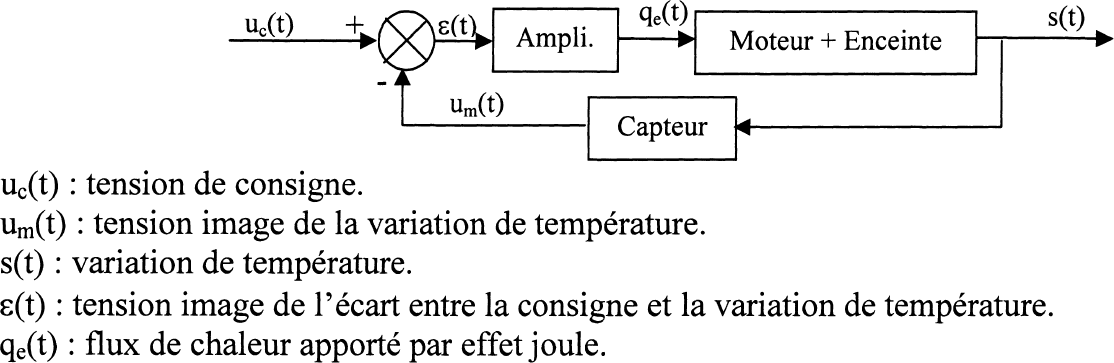
\includegraphics[width=\linewidth]{66_01}
\end{marginfigure}


L'ensemble \{Moteur + enceinte \} est modélisé par un premier ordre de fonction de transfert $H(p)=\dfrac{H_0}{1+\tau p}$
avec $H_0 = \SI{0}{\degres C.W^{-1}}$ et $\tau=\SI{200}{s}$?

Le capteur es tmodélisé par un système de fonction de transfert $\beta \exp^{-T_r p}$ avec $\beta = \dfrac{5}{200}\si{V.\degres C^{-1}}$ et $T_r = \SI{20}{s}$.

L'amplificateur est modélisé par un gain pur $A= \SI{400}{W.V^{-1}}$

Le cahier des charges est le suivant. 

\begin{marginfigure}
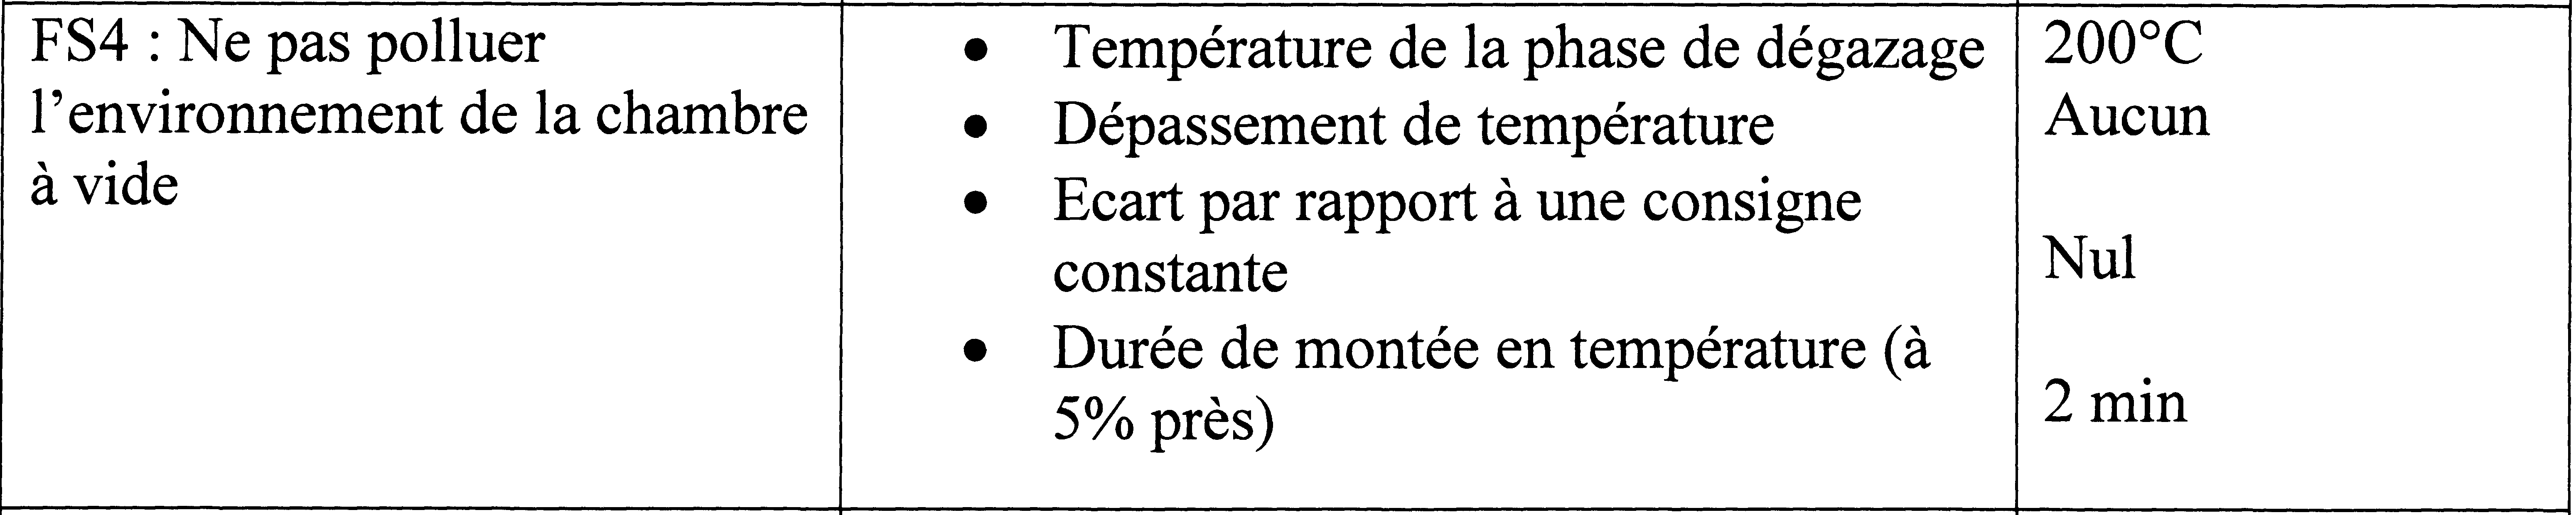
\includegraphics[width=\linewidth]{66_02}
\end{marginfigure}
\fi

\question{Expliquez en quelques lignes pourquoi le retard engendé par le capteur risque de rendre le système non conforme au cahier des charges.}
\ifprof
\else 
\fi


\ifprof
\else 
Pour supprimer l'inflience du retard, on choisit d'unsatller un correcteur en série juste avant l'amplificateur, comme indiqué sur le schéma-blocs suivant. 

\begin{marginfigure}
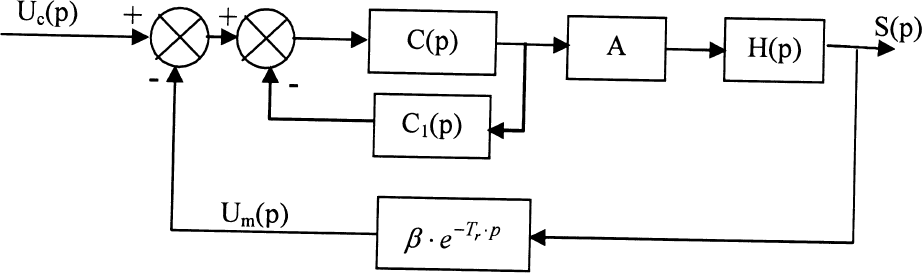
\includegraphics[width=\linewidth]{66_03}
\end{marginfigure}
\fi

\question{Déterminer l'expression littérale de la fonction de transfert en boucle fermée du système ainsi corrigé en fonction de $H(p)$, $A$, $C(p)$, $C_1(p)$, $\beta$ et $T_r$.}
\ifprof
\else 
\fi

\question{Déterminer l'expression de $C_1(p)$ en fonction de $H(p)$, $A$, $\beta$ et $T_r$, pour que le système ait un comportement équivalent au système sans retard suivant.}
\ifprof
\else 
\fi

\ifprof
\else 

\begin{marginfigure}
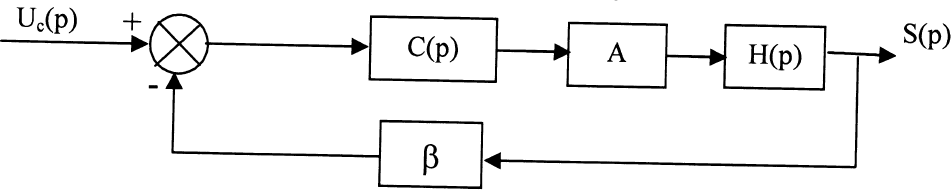
\includegraphics[width=\linewidth]{66_04}
\end{marginfigure}

Grâce au correcteur $C(p)$ choisi précédemment, le retard n'a plus d'influence sur la commande du système. 

On choisit comme fonction de transfert de la seconde partie du ocrrecteur $C(p)=K_i \dfrac{1+T_i p}{T_i p}$. 
\fi

\question{Justifier le choix de $C(p)$ en vous appuyant sur les exigences du cahier des charges.}
\ifprof
\else 
\fi

\question{Déteminer l'expression de la fonction de transfert en boucle fermée $F(p)=\dfrac{S(p)}{U_c(p)}$ du système en fonction de $K_i$ et $T_i$.}
\ifprof
\else 
\fi

\question{Calculer la valeur de $T_i$ pour que le système se comporte comme un premier ordre.}
\ifprof
\else 
\fi

\question{Calculer la valeur de $K_i$ pour que le temps de montée en température soit compatible avec les données du cahier des charges.}
\ifprof
\else 
\fi


\ifprof
\else

\noindent\footnotesize
 \fbox{\parbox{.9\linewidth}{
Éléments de corrigé : 
\begin{enumerate}
\item .
\item $H_{\text{BF corrigee}} = \dfrac{AHC}{1+CC_1+AHC\beta \exp^{-T_r p}}$.
\item $C_1=AH\beta \left( 1- \exp^{-T_r p}\right)$.
\item .
\item $F(p)=\dfrac{AH_0K_i\left(1+T_i p\right)}{\left(1+\tau p\right)T_i p+A\beta H_0K_i \left(1+T_i p\right)}$.
\item $T_i = \tau$.
\item $K_i  = \dfrac{\tau }{40 A\beta H_0} = 25$.
\end{enumerate}}}
\normalsize


\marginnote{Corrigé voir \ref{COR:03::66}.}

\fi 
 
\graphicspath{{\repStyle/png/}{../COR/COR-03-PI/67_PompeTurbo/images/}} 
\normaltrue \difficilefalse \tdifficilefalse
\correctionfalse
%\UPSTIidClasse{11} % 11 sup, 12 spé
%\newcommand{\UPSTIidClasse}{11}

\exer{Pompe turbo-moléculaire $\star$ \label{COR:03::67}}
% CCS PSI 2009
\setcounter{question}{0}\marginnote{\xpComp{COR}{03}}%\UPSTIcompetence[2]{C2-04}
\index{Compétence C2-04}\index{Compétence COR-03}
\index{Correcteur}
\index{Correcteur proportionnel intégral}
\index{Pompe turbo-moléculaire}


\ifcorrection
\else
\marginnote{\textbf{Pas de corrigé pour cet exercice.}}
\fi
\ifprof
\else 

Afin de satisfaire les critères du cahier des charges, on envisage d'asservir le
palier magnétique par un premier bouclage de stabilisation (retour $K_D p + K_P$).
Un second retour unitaire associé à un correcteur $C(p)$ assure la régulation en
position du palier. On utilisera par la suite les paramètres suivants : 
$K_e = \SI{5000}{V.m^{-1}}$, $K_0 = \SI{190}{N.m^{-1}}$ et $m=\SI{10}{kg}$.
On considère dans un premier temps le système sans correction : $C(p)=1$.

\begin{marginfigure}
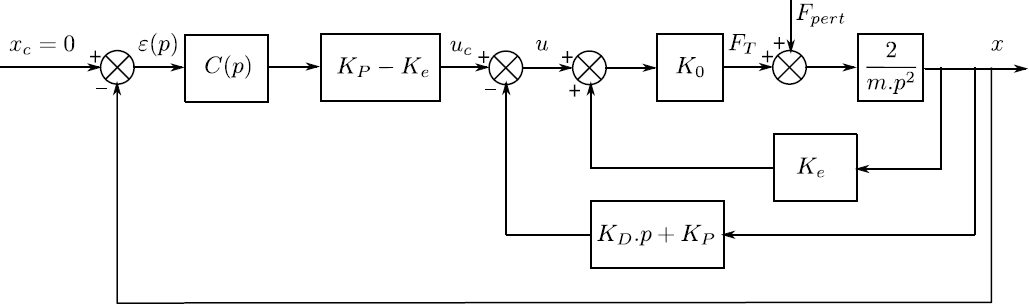
\includegraphics[width=\linewidth]{67_01}
\end{marginfigure}

\begin{marginfigure}
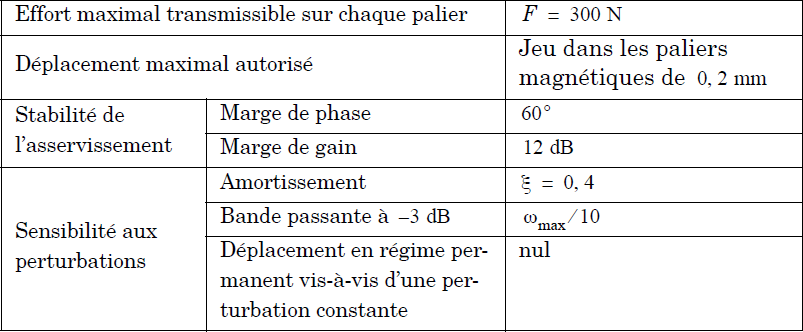
\includegraphics[width=\linewidth]{67_02}
\end{marginfigure}
\fi

\question{Déterminer la fonction de transfert de la boucle interne $H_{\text{PM I}}(p)=\dfrac{X(p)}{\varepsilon(p)}$, en fonction de $K_e$, $K_0$, $m$, $K_P$ et $K_D$. Préciser les conditions
sur $K_D$ et $K_P$ pour que $H_{\text{PM I}}(p)$ soit stable en boucle ouverte.}
\ifprof
\else 
\fi

\question{En considérant l’ensemble de l’asservissement, déterminer la fonction de transfert $H_{\text{pert}}(p)=\dfrac{X(p)}{F_{\text{pert}}(p)}$, puis calculer les valeurs de $K_D$ et $K_P$
permettant de respecter les spécifications du cahier des charges en terme de bande passante et d'amortissement.}
\ifprof
\else 
\fi

\ifprof
\else 
\begin{marginfigure}
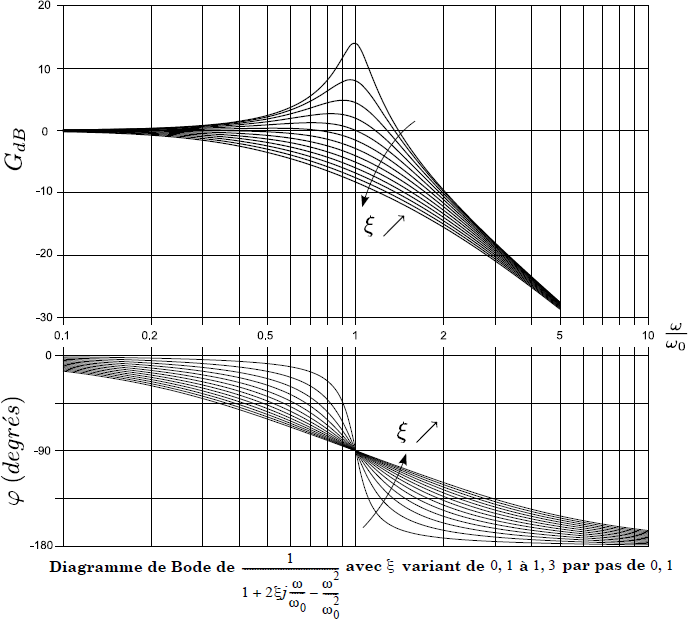
\includegraphics[width=\linewidth]{67_03}
\end{marginfigure}
\fi

\question{Tracer l'allure des diagrammes de Bode asymptotique et réel de la fonction
de transfert de la boucle interne $H_{\text{PM I}}(p)$ et préciser la pulsation de coupure
ainsi que les marges de gain et de phase. Valider les critères de stabilité du
cahier des charges.}
\ifprof
\else 
\fi

\ifprof
\else 
L'ouverture et la fermeture des arrivées de gaz sont assurées par des « vannes
guillotines ». À la suite de la fermeture de la guillotine, le palier est soumis à un
effort bref mais violent, qui peut être modélisé par une perturbation d'effort en
échelon d'amplitude $F_G$.
\fi

\question{Conclure quant au critère de sensibilité vis-à-vis des perturbations.}
\ifprof
\else 
\fi

\ifprof
\else 
Afin d'améliorer les performances du système, on utilise un correcteur de fonction
de transfert : $C(p)=K_i \left( 1+\dfrac{1}{T_i p}\right)$.
\fi

\question{Quelle performance est directement améliorée par ce correcteur ? (justifier
votre réponse sans calcul).}
\ifprof
\else 
\fi

\question{Tracer l'allure du diagramme de Bode du correcteur en précisant les
valeurs caractéristiques. Expliquer comment choisir $K_i$ et $T_i$ afin de conserver
des marges de gain, de phase, et une pulsation de coupure proches de celles obtenues
sans correction ($C(p)=1$ ). Proposer des valeurs numériques.}
\ifprof
\else 
\fi

\ifprof
\else 

On admet que le correcteur influe peu sur le temps de réponse et les dépassements
lorsque les marges de stabilité et la pulsation de coupure sont conservées.
On garde par conséquent les valeurs de $K_P$ et $K_D$ obtenues précédemment.

Conclusion : nous avons donc désormais dimensionné les deux boucles d'asservissement
successives permettant d'obtenir les performances attendues du palier
magnétique.

Afin de préparer la prochaine partie, relative à l'étude dynamique du rotor, on
recherche un modèle simple de l'effort du palier magnétique actif en fonction du
déplacement $x$ de l'arbre, dans une gamme de vitesses de rotation raisonnables
variant de $\SI{10000}{tr.min^{-1}}$ à $\SI{30000}{tr.min^{-1}}$.
\fi


\question{Déterminer la fonction de transfert $K(p)$ telle que $F_T(p)=K(p)X(p)$.
À partir de simplifications justifiées, montrer que dans la plage de fréquences
considérée, l'effort $F_T(p)$ peut s'écrire sous la forme d'un modèle ressort amortisseur
$F_T(t)=-kx(t)-c\dot{x}(t)$ où vous préciserez les valeurs numériques de $k$ et $c$. Comment évolue le modèle lorsque $\omega$ augmente au delà de cette plage de
fréquences ?}
\ifprof
\else 
\fi



\ifprof
\else

\noindent\footnotesize
 \fbox{\parbox{.9\linewidth}{
Éléments de corrigé : 
\begin{enumerate}
\item $K_P>K_e$ et $K_D>0$.
\item $K_P = 5900$ et $K_D = 5,5$.
\item $\omega_{\text{c0}}=\SI{150}{rad.s^{-1}}$, $M_{\varphi}=\SI{110}{\degres}$.
\item .
\item .
\item $K_i=1$ et $T_i = \SI{0,07}{s}$.
\item .
\end{enumerate}}}
\normalsize


\marginnote{Corrigé voir \ref{COR:03::67}.}

\fi 
 
\graphicspath{{\repStyle/png/}{../COR/COR-03-PI/68_Roburoc/images/}} 
\normaltrue \difficilefalse \tdifficilefalse
\correctionfalse
%\UPSTIidClasse{11} % 11 sup, 12 spé
%\newcommand{\UPSTIidClasse}{11}

\exer{Roburoc $\star$ \label{COR:03::68}}
%% CCMP 2009
\setcounter{question}{0}\marginnote{\xpComp{COR}{03}}%\UPSTIcompetence[2]{C2-04}
\index{Compétence C2-04}\index{Compétence COR-03}
\index{Correcteur}
\index{Correcteur proportionnel intégral}
\index{Roburoc}


\ifcorrection
\else
\marginnote{\textbf{Pas de corrigé pour cet exercice.}}
\fi

\ifprof
\else

Soit le schéma-blocs suivant. 

\begin{marginfigure}
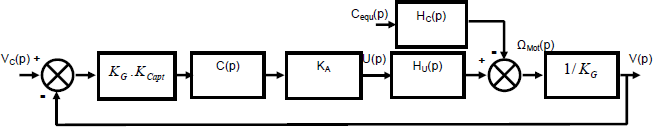
\includegraphics[width=\linewidth]{68_01}
\end{marginfigure}

On a $H_U(p) = \dfrac{K_U}{\left( T_1 p +1 \right)\left( T_2 p +1 \right)}$ et $H_C(p) = \dfrac{K_C \left( 1+\dfrac{L}{r}p\right)}{\left( T_1 p +1 \right)\left( T_2 p +1 \right)}$. $K_U =\SI{8,3}{rad.s^{-1}.V^{-1}}$, $K_C = \SI{152,7}{rad.s^{-1}.N^{-1}.m^{-1}}$, $T_1 = \SI{2,1}{ms}$ et $T_2 = \SI{0,36}{ms}$.

\textbf{Etude des performances sans correction : $C( p) =1$}

Nous distinguerons dans la suite :
\begin{itemize}
\item l’étude en poursuite : le couple de perturbation équivalent $C_{\text{equ}} (t)$ est nul. $V_c(t)$ varie ;
\item l’étude en régulation : la vitesse de consigne de la plate-forme $V_c(t)$  est nulle. $C_{\text{equ}} (t)$ varie.
\end{itemize}

Les diagrammes de Bode de la Fonction de Transfert en Boucle Ouverte $\text{FTBO}( p)$ non corrigée sont fournis pour $C( p) = 1$.

\begin{marginfigure}
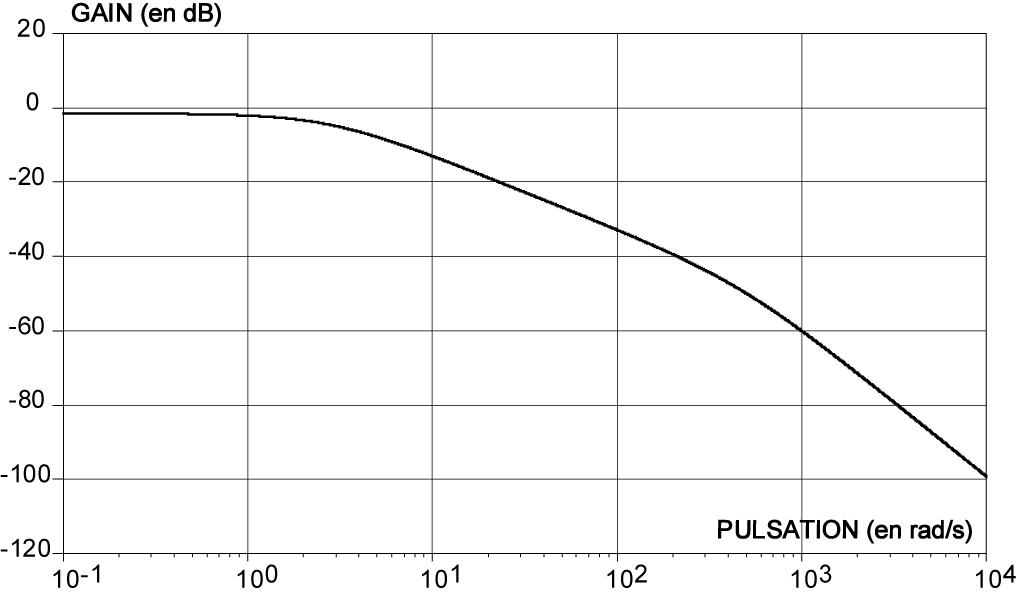
\includegraphics[width=\linewidth]{68_02}
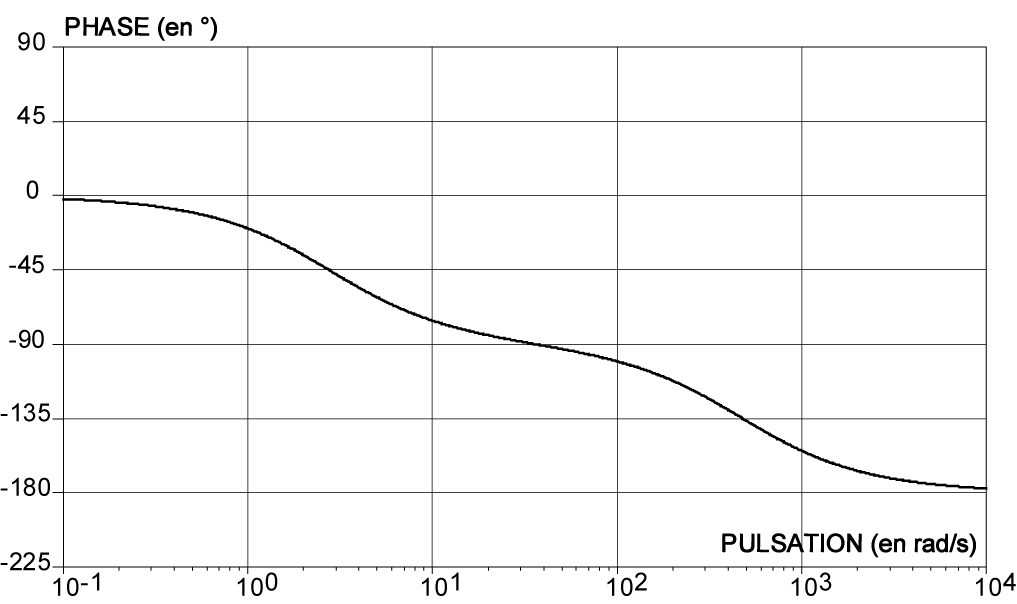
\includegraphics[width=\linewidth]{68_03}
\end{marginfigure}
\fi

\question{Le système étudié est-il stable théoriquement ? Justifier vos réponses.}
\ifprof
\else 
\fi

\question{Etudier l’aptitude du système sans correction à respecter les critères de précision. Vous déterminerez
notamment les expressions littérales de l’erreur statique en poursuite pour une consigne de vitesse de la
plate-forme $V_c (t)$ en échelon d’amplitude $V_{\text{CO}}$ : $V_C(t) = V_{\text{CO}}  u(t)$ (avec $u(t)$ l’échelon unitaire) et de l’influence en régulation d’une perturbation $C_{\text{equ}} (t)$ en échelon d’amplitude $C_0$, sur la vitesse réelle $V (t)$ de la plate-forme en régime permanent.}
\ifprof
\else 
\fi

\textbf{Etude des performances avec un correcteur de fonction de transfert : $C(p)=\dfrac{K_I}{p}$}

\question{Indiquer quelle est la nature de la correction effectuée par ce correcteur (ou désignation du correcteur) ?
Indiquer pour quelle(s) raison(s) principale(s) ce correcteur a été choisi. Valider ce choix vis à vis du cahier
des charges. Sans calcul, donner l’influence de ce correcteur sur les autres performances attendues.}
\ifprof
\else 
\fi

Reprenons le diagramme de Bode précédent.

\question{Compléter le document-réponse en traçant les diagrammes de Bode du
correcteur avec $K_I = \SI{1}{s^{-1}}$ . Déterminer alors la valeur de $K_I$ maximale notée $K_{\text{I max}}$ permettant de respecter les marges de stabilité énoncées dans le cahier des charges.}
\ifprof
\else 
\fi

\ifprof
\else
Afin d’évaluer analytiquement le temps de réponse à 5\%, Il est proposé d’adopter une modélisation simplifiée du
comportement du moteur en conservant uniquement le mode associé au pôle << dominant >>. On donne $T_{5\% \text{mini}}\cdot \omega_0 = 3$ avec $\omega_0$ la pulsation propre non amortie d’un système fondamental du second ordre.
\fi

\question{En analysant les valeurs numériques des pôles de la fonction de transfert du moteur en poursuite $H_U( p)$,
préciser quel est le pôle dominant et proposer alors un modèle simplifié de la fonction de transfert $H_U ( p)$.
Déterminer alors la valeur numérique de $K_I$ notée $K_{I\SI{5}{\%}}$ minimisant le temps de réponse à 5\% pour une
entrée échelon en poursuite. Calculer alors la valeur approchée du temps de réponse à 5\% minimale $T_{5\% \text{mini}}$ et comparer la au cahier des charges.}
\ifprof
\else 
\fi

\textbf{Etude des performances avec un correcteur proportionnel intégral : $C(p)=K_P \left( 1+\dfrac{1}{T_i p}\right)$}

\ifprof
\else
Le correcteur est remplacé par un correcteur proportionnel intégral. Des réponses temporelles du système corrigé sont
tracées avec :
\begin{itemize}
\item une consigne de vitesse unitaire de la plate-forme $V_c (t)= u(t)$ (avec $u(t)$ l’échelon unitaire) ;
\item une perturbation sous la forme d’un échelon unitaire retardé de 5 secondes $C_{\text{equ}} (t) = u(t - 5)$ ;
\item un gain du correcteur $K_P= 1$ ;
\item différentes valeurs de $T_I$.
\end{itemize}

\begin{marginfigure}
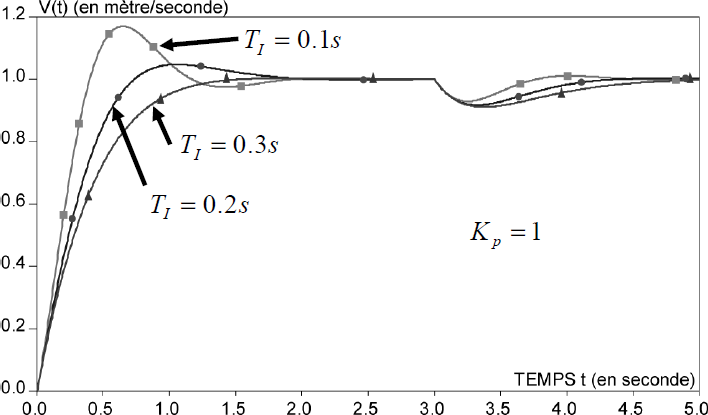
\includegraphics[width=\linewidth]{68_04}
\end{marginfigure}
\fi

\question{Parmi les différentes valeurs de $T_I$ , choisir celle qui assure le temps de réponse à 5\% le plus faible. Vous
ferez apparaître ce temps de réponse sur la figure.}
\ifprof
\else 
\fi


\ifprof
\else 
La valeur de $T_I$ déterminée à la question précédente est retenue pour le réglage du correcteur proportionnel intégral.
Il s’agit alors de choisir le gain du correcteur $K_p$ à partir des simulations proposées.

\begin{marginfigure}
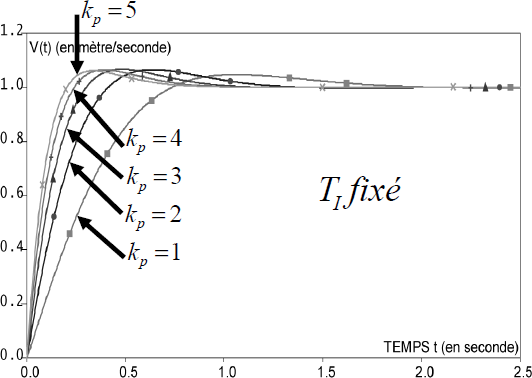
\includegraphics[width=\linewidth]{68_05}
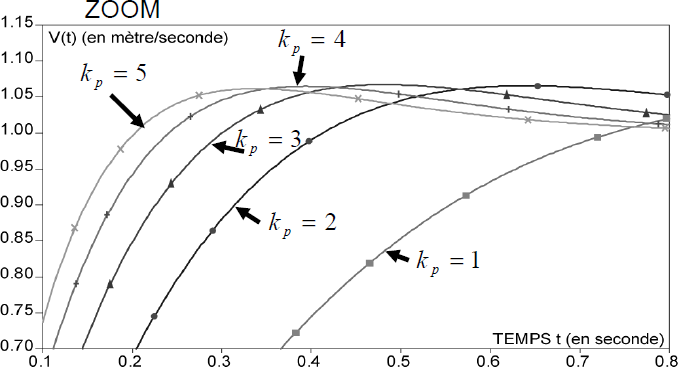
\includegraphics[width=\linewidth]{68_06}
\end{marginfigure}
\fi

\question{Parmi les différentes valeurs de $K_p$ , choisir la valeur qui assure un temps de réponse à 5\% au plus près de
la valeur fournie dans le cahier des charges.}
\ifprof
\else 
\fi

\ifprof
\else 

Avec le couple de valeurs ($T_I$ et $K_p$) obtenu, la réponse fréquentielle du système en boucle ouverte a été tracée.
\begin{marginfigure}
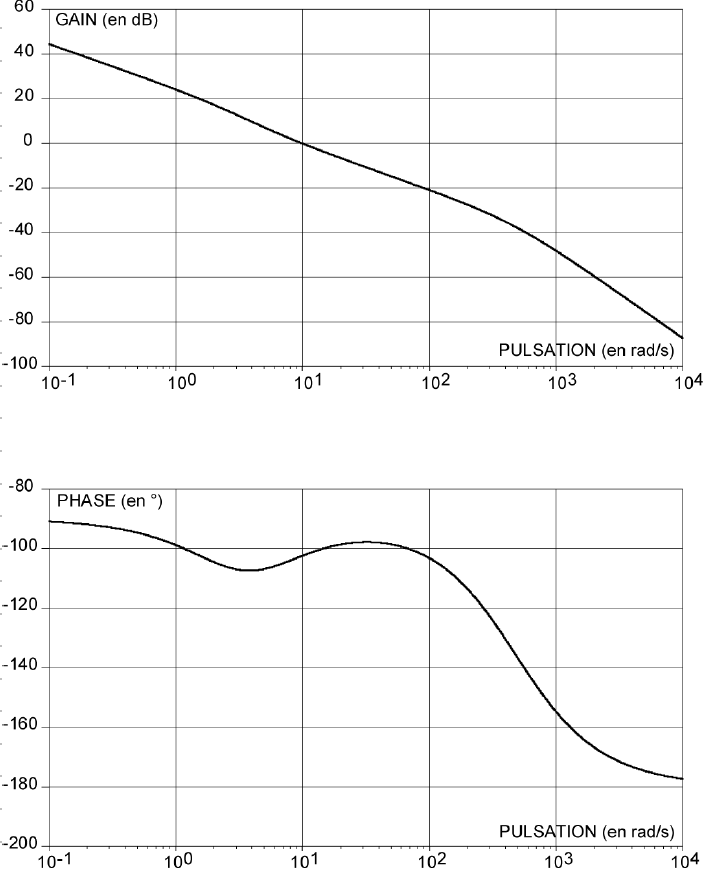
\includegraphics[width=\linewidth]{68_07}
\end{marginfigure}
\fi


\question{Conclure quant à la capacité de ce correcteur à respecter tous les critères du cahier des charges.}
\ifprof
\else 
\fi


\ifprof
\else

\noindent\footnotesize
 \fbox{\parbox{.9\linewidth}{
Éléments de corrigé : 
\begin{enumerate}
\item .
\end{enumerate}}}
\normalsize


\marginnote{Corrigé voir \ref{COR:03::68}.}

\fi 
 
\graphicspath{{\repStyle/png/}{../COR/COR-03-PI/70_Hublex/images/}} 
\normaltrue \difficilefalse \tdifficilefalse
\correctionfalse
%\UPSTIidClasse{11} % 11 sup, 12 spé
%\newcommand{\UPSTIidClasse}{11}

\exer{Hublex $\star$ \label{COR:03::68}}
%% CCINP MP 2020
\setcounter{question}{0}\marginnote{\xpComp{COR}{03}}%\UPSTIcompetence[2]{C2-04}
\index{Compétence C2-04}\index{Compétence COR-03}
\index{Correcteur}
\index{Correcteur proportionnel intégral}
\index{Hublex}


\ifcorrection
\else
\marginnote{\textbf{Pas de corrigé pour cet exercice.}}
\fi



\ifprof
\else

L’architecture retenue pour contrôler le couple moteur est un asservissement en intensité, image du
couple moteur (voir équation précédente). Le schéma-blocs est représenté \autoref{fig_13}. Un convertisseur IU
fournit au calculateur une tension $\indice{u}{ic}(t)$ image de l’intensité de consigne $i_c(t)$, proportionnelle à cette
dernière de coefficient $\indice{K}{iu}$. De même, l’intensité réelle $i(t)$, mesurée par un capteur d’intensité de
coefficient $\indice{K}{capt}$, a pour image $\indice{u}{im}(t)$. L’écart, noté $\varepsilon(t) = \indice{u}{ic}(t) - \indice{u}{im}(t)$, est traité par le correcteur de fonction de transfert $C(p)$, qui impose la tension $u(t)$ aux bornes du moteur.
%On note $I_c(p)$, $\indice{U}{ic}(p)$, $\indice{U}{im}(p)$, $\varepsilon(p)$ les transformées de Laplace respectives de $i_c(t)$, $\indice{u}{ic}(t)$, $\indice{u}{im}(t)$ et $\varepsilon(t)$.

On donne la fonction de transfert du moteur : $H_m(p)=K_m\dfrac{1+\tau_m p}{1+\dfrac{2z_m}{\omega_{0m}}p+\dfrac{1}{\omega_{0m}^2}p^2}$.


\begin{marginfigure}
\marginfigureing
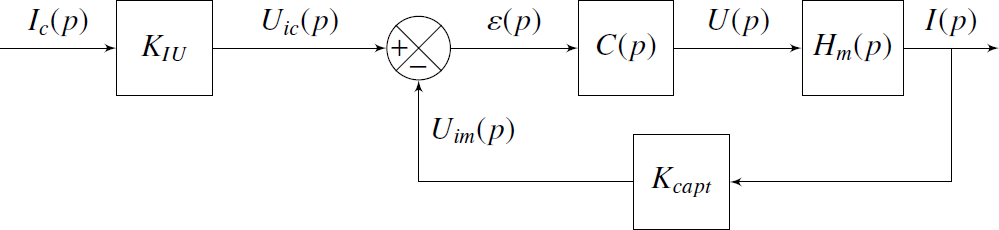
\includegraphics[width=\linewidth]{fig_13}
\caption{Schéma-blocs \label{fig_13}}
\end{marginfigure}

\fi

\question{Préciser, en justifiant, quelle valeur donner à $\indice{K}{iu}$, caractéristique du convertisseur IU.}


\ifprof
\else
On prend, dans un premier temps, un correcteur purement proportionnel: $C(p)=K_p$.

On en déduit la fonction de transfert $H_I(p)=\dfrac{I(p)}{I_c(p)}$ :

$H_I(p)=\dfrac{K'}{1+K'}\dfrac{1+\tau_m p}{1+  
\dfrac{\dfrac{2z_m}{\omega_{0m}}+ K'\tau_m}{1+K'}p 
+ \dfrac{1}{\omega_{0m}^2(1+K')} p^2}$, avec $K'=\indice{K}{iu}K_pK_m$.

\fi

\question{Calculer l’expression littérale de l’erreur en régime permanent notée $\mu_s$, pour une entrée indicielle (i.e. $I_c(p)$ est un échelon unitaire), en fonction de $\indice{K}{iu}$, $\indice{K}{p}$ et $K_m$.}

La \autoref{fig_14} présente les diagrammes de Bode en boucle ouverte de l’asservissement étudié, en prenant $K_p=10$.


%Q30.
\question{Conclure, lorsque cela est possible, quant au respect des sousexigences de l’exigence «~1.7.1.1~» avec ce type de correcteur.}

Dans un deuxième temps, il est décidé d’utiliser un correcteur de type proportionnel intégral. Sa fonction de transfert est notée : $C(p)=K_p+\dfrac{K_i}{p}$.

%Q31.
\question{Préciser l’influence de cecorrecteur sur les performances du système. Justifier le choix de ce type de correcteur dans le cas étudié.}

On souhaite régler le correcteur afin de respecter les performances de précision et de stabilité.

%Q32.
\question{Tracer sur le DR4, les diagrammes de Bode asymptotique du correcteur, ainsi que l’allure des courbes réelles pour $K_p=10$ et $K_i=1000$. On précisera les valeurs numériques associées aux valeurs caractéristiques. On se propose de régler le correcteur grâce à la méthode suivante, en deux étapes :}
\textit{\begin{enumerate}
\item réglage de $K_p$ seul (c’est-à-dire en considérant $K_i=0$ tout d’abord), de façon à respecter les exigences de stabilité et de bande passante;
\item  réglage de $K_i$ de façon à éloigner la pulsation de cassure du correcteur à une décade vers la gauche de la pulsation de coupure à \SI{0}{dB}, de manière à ce que $\SI{0}{dB}$ ne soit quasiment pas modifiée.
\end{enumerate}}

%Q33.
\question{En suivant cette méthode, déterminer en justifiant la valeur numérique de $K_p$.}

%Q34.
\question{Déterminer alors la valeur numérique de $K_i$.}

 Une fois le correcteur réglé, on obtient les diagrammes de Bode en boucle ouverte (\autoref{fig_15}) et les réponses temporelles (\autoref{fig_16}), pour un échelon d’intensité $i_c(t)$ de \SI{2}{A}.

% Q35.
\question{Commenter le résultat obtenu vis-à-vis de l’exigence «~1.7.1.1.4~». Expliquer pourquoi, à partir des exigences du D6, cet asservissement n’est pas directement implanté en l’état dans le système.}

\ifprof
\else

Le correcteur reste inchangé. Afin de palier au problème identifié précédemment, on apporte une dernière évolution au sein du calculateur. Cela permet de respecter les exigences de l’asservissement. \autoref{fig_17} présente les réponses temporelles du système pour un échelon d’intensité $i_c(t)$ de \SI{2}{A}.
\fi

%Q36.
\question{Préciser quelle ultime modification a apporté le constructeur afin de respecter les exigences de l’asservissement.}


\ifprof
\else
\begin{marginfigure}
\marginfigureing
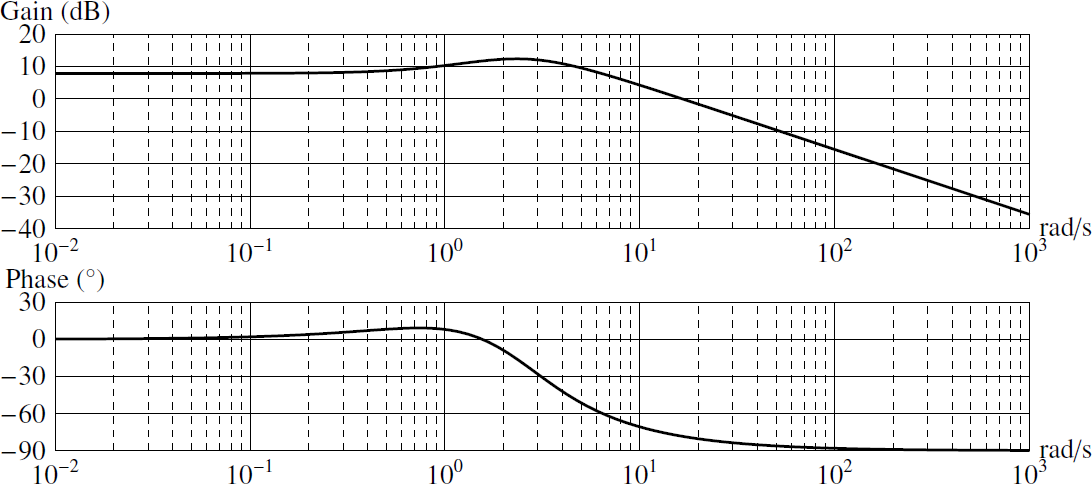
\includegraphics[width=\linewidth]{fig_14}
\caption{Diagrammes de Bode en boucle ouverte pour $K_p = 10$\label{fig_14}}
\end{marginfigure}


\begin{marginfigure}
\marginfigureing
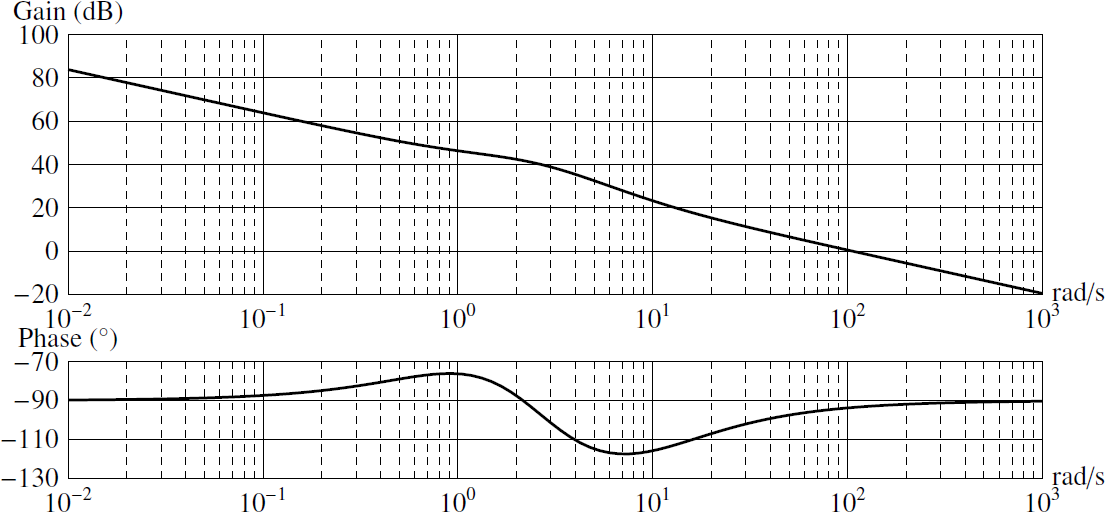
\includegraphics[width=\linewidth]{fig_15}
\caption{Diagrammes de Bode en boucle ouverte avec réglage du correcteur PI effectué \label{fig_15}}
\end{marginfigure}

\begin{marginfigure}
\marginfigureing
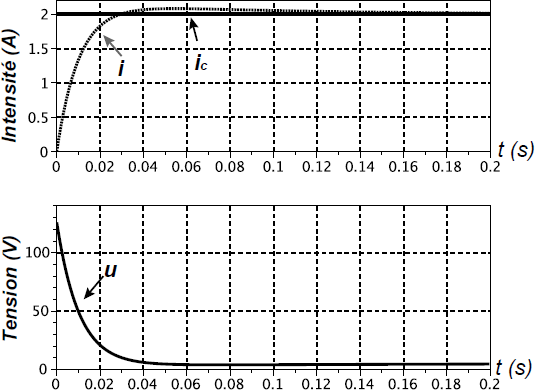
\includegraphics[width=.95\linewidth]{fig_16}
\caption{Réponses temporelles avec réglage du correcteur PI effectué \label{fig_16}}
\end{marginfigure}


\begin{marginfigure}
\marginfigureing
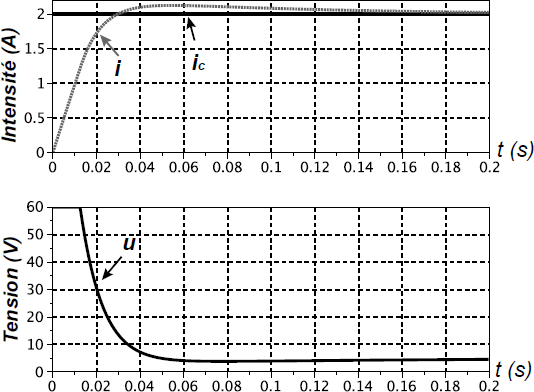
\includegraphics[width=.95\linewidth]{fig_17}
\caption{Réponses temporelles du système finalement implanté\label{fig_17}}
\end{marginfigure}
\fi


\ifprof
\else



\marginnote{Corrigé voir \ref{COR:03::70}.}

\fi 
 
\section{Régler un correcteur à avance de phase} 
\graphicspath{{\repStyle/png/}{../COR/COR-04-AP/65_Eclipse_03/images/}} 
\normaltrue \difficilefalse \tdifficilefalse
\correctionfalse
%\UPSTIidClasse{11} % 11 sup, 12 spé
%\newcommand{\UPSTIidClasse}{11}

\exer{Système éclipse $\star$ \label{COR:04:C2:04:65:02}}
% Banque PT SI A 2009
\setcounter{question}{0}
\marginnote{\xpComp{COR}{°4}}
%\UPSTIcompetence[2]{C2-04}
\index{Compétence C2-04}
\index{Compétence COR-04}
\index{Correcteur}
\index{Correcteur avance de phase}
\index{Système éclipse}


\ifcorrection
\else
\marginnote{\textbf{Pas de corrigé pour cet exercice.}}
\fi
\ifprof
\else 

Le schéma-blocs sous la forme suivante avec un gain unitaire pour le capteur
de vitesse.

\begin{marginfigure}
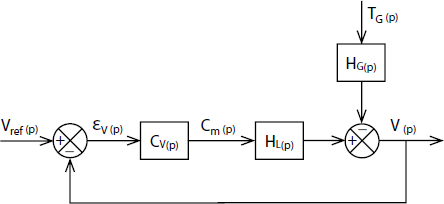
\includegraphics[width=\linewidth]{65_01}
\end{marginfigure}

$H_L(p)=\dfrac{K_L}{1+\tau_L p}$ et $H_G(p)=\dfrac{K_G}{1+\tau_G p}$  avec $\tau_G=\tau_L = \SI{20}{ms}$, $K_L = \SI{1e-3}{N^{-1}s^{-1}}$ et $K_G = \SI{2e-5}{mN^{-1}s^{-1}}$.


Le cahier des charges donne les valeurs des critères d'appréciation adoptés :
\begin{itemize}
\item la précision : en régime permanent à vitesse constante, soit $\varepsilon_S=0$ et à accélération constante, soit $\varepsilon_T=0$; $\varepsilon_S$ désigne l'erreur statique de position et $\varepsilon_T$ l'erreur statique de vitesse ou erreur de traînage;
\item la rapidité : le temps de réponse à \SI{5}{\%} tel que : $t_{\text{R}\SI{5}{\%}}\leq \SI{1}{s}$;
\item la stabilité : marge de phase $\geq \SI{45}{\degres}$ et marge de gain $\geq \SI{10}{dB}$.
\end{itemize}

On considère que le système n'est pas perturbé et que $T_G(p)=0$.
On choisit une correction telle que $C_{V}(p)= C_{V1}(p) \cdot C_{V2}(p) $ avec $C_{V1}(p)=\dfrac{K_i}{p^2}$ et $C_{V2}(p)=\dfrac{1+k_f \tau_v p }{1+\tau_v p }$ où $k_f$ est appelé coefficient de filtrage et dont la valeur est généralement comprise entre $5\leq k_f \leq 10$.
\fi

\question{Comment se nomme la correction apportée par $C_{V2}(p)$ ? Expliquer brièvement comment ce type de correction
permet de stabiliser un système instable. Pour cela, tracer l'allure du diagramme de Bode correspondant à ce
terme.}
\ifprof
\else 
\fi


\ifprof
\else 
La figure suivante fournit les diagrammes de Bode du système corrigé uniquement par le correcteur 
$C_{V1}(p)$ avec $K_V=1$, c'est-à-dire la fonction de transfert $W(p) =\dfrac{1}{p^2}H_L(p)$.


\begin{marginfigure}
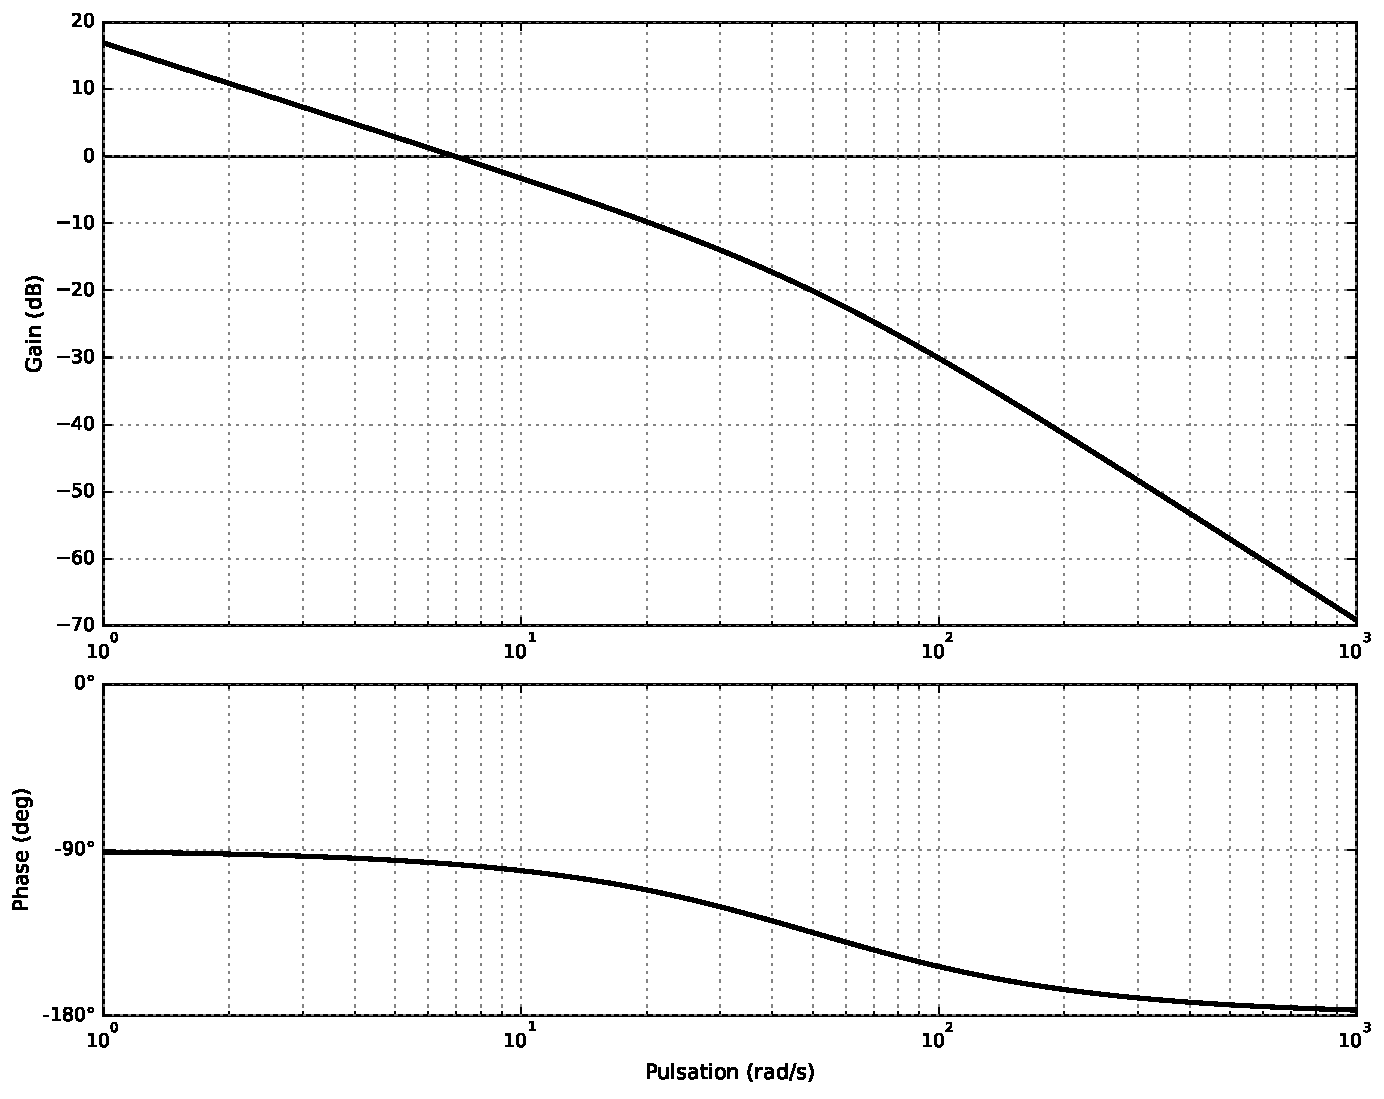
\includegraphics[width=\linewidth]{65_02}
\end{marginfigure}
\fi

\question{Lire sur les diagrammes de Bode du système de fonction de transfert $W(p)$, la valeur de la
pulsation de coupure $\omega_{\SI{0}{dB}}$ où le rapport d'amplitude $A_{\text{dB}}$ s'annule. Quelle est, à cette pulsation, la valeur de la
phase ? Justifier alors la présence de la correction $\dfrac{1+k_f \tau_v p }{1+\tau_v p }$}
\ifprof
\else 
\fi

\question{Exprimer en fonction de $\tau_V$ et de $k_f$ la pulsation $\omega_m$ pour laquelle la phase maximale est atteinte. On rappelle pour cela que $\dfrac{\dd \arctan x}{\dd x}=\dfrac{1}{1+x^2}$.}
\ifprof
\else 
\fi

\ifprof
\else 
On montre que pour un coeffcient de filtrage $k_f=8$, la valeur maximale de la phase, ajoutée par la correction,
est de $\SI{51}{\degres}$.

On choisit de prendre pour $\omega_m$ la valeur de la pulsation pour laquelle le système corrigé uniquement par le
correcteur $C_{V1}(p)$ , possède une phase de $-\SI{185}{\degres}$.
\fi

\question{Lire sur les diagrammes de Bode la valeur de $\omega$ pour laquelle la phase du système corrigé
uniquement par le correcteur $C_{V1}(p)$, est de $-\SI{185}{\degres}$. En déduire la valeur de $\tau_V$ correspondante.}
\ifprof
\else 
\fi

\question{Pour la valeur de $\tau_V$ trouvée précédemment, on donne le diagramme de Black (hors programme...) de
la FTBO du système corrigé entièrement, obtenu pour $K_V=75$. Donner la valeur de $K_V$ qui maximise la marge de
phase en expliquant comment vous l'obtenez à la lecture de ce diagramme.
Valider alors les performances attendues en terme de stabilité.}
\ifprof
\else 
\fi

\ifprof
\else 
\begin{marginfigure}
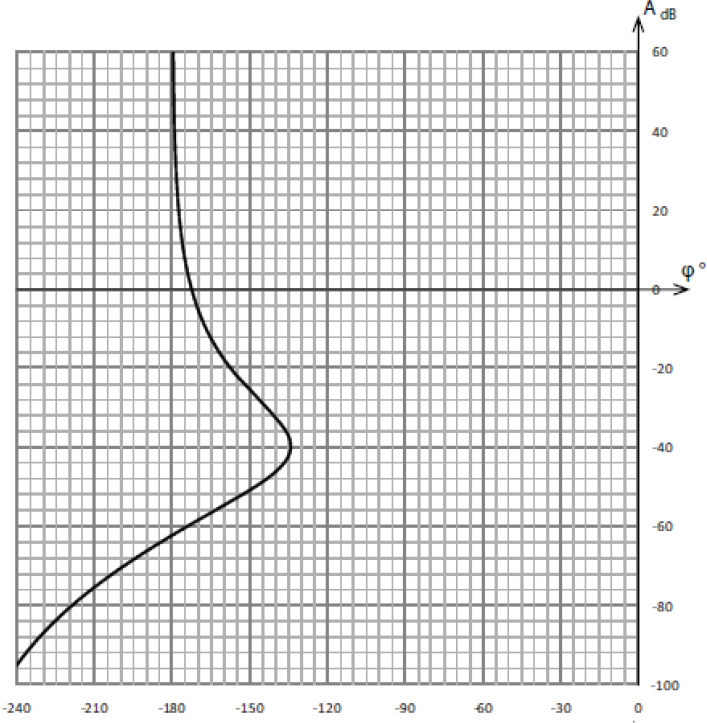
\includegraphics[width=\linewidth]{65_03}
\end{marginfigure}
\fi

\question{On donne le tracé de la réponse temporelle à un échelon de vitesse de $\SI{10}{mm.s^{-1}}$
du système corrigé pour trois valeurs de $K_V$. Quelle valeur de $K_V$ permet de valider les performances attendues
en terme de rapidité ? Donnez une valeur optimale de $K_V$ qui permette de satisfaire au mieux le cahier des
charges ? }
\ifprof
\else 
\fi

\ifprof
\else 
\begin{marginfigure}
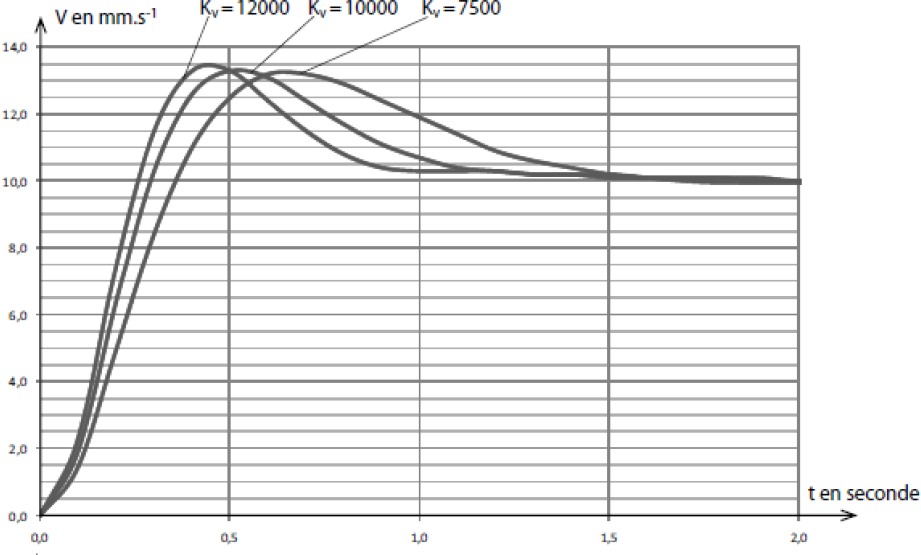
\includegraphics[width=\linewidth]{65_04}
\end{marginfigure}
\fi


\question{Le système ainsi corrigé est-il robuste aux perturbations en échelon mais également en rampe comme celles
provoquées par le système de maintien en tension ?}
\ifprof
\else 
\fi

\ifprof
\else
\marginnote{Corrigé voir \ref{COR:04:C2:04:65:02}.}
\fi 
 
\section{Modéliser un correcteur numérique} 
\section{Implanter un correcteur sur une cible} 
